\chapter{Étude conceptuelle}
\label{chap:etude_conceptuelle}

\section{Introduction}

Après avoir exposé les besoins et les exigences fonctionnelles, ce chapitre présente la conception conceptuelle d'Alpha Store. Nous distinguons la vue statique, qui montre la structure du système, et la vue dynamique, qui illustre les interactions et les comportements dans le temps.

\section{Conception : vue statique}

La vue statique décrit l'architecture globale et les relations entre les principaux composants logiciels et matériels.

\subsection{Diagramme de déploiement}

Le diagramme de déploiement représente les nœuds physiques ainsi que les composants logiciels qui y sont déployés, notamment le serveur Apache/PHP, la base de données MariaDB et les services Python pour l'IA.

\begin{figure}[H]
    \centering
    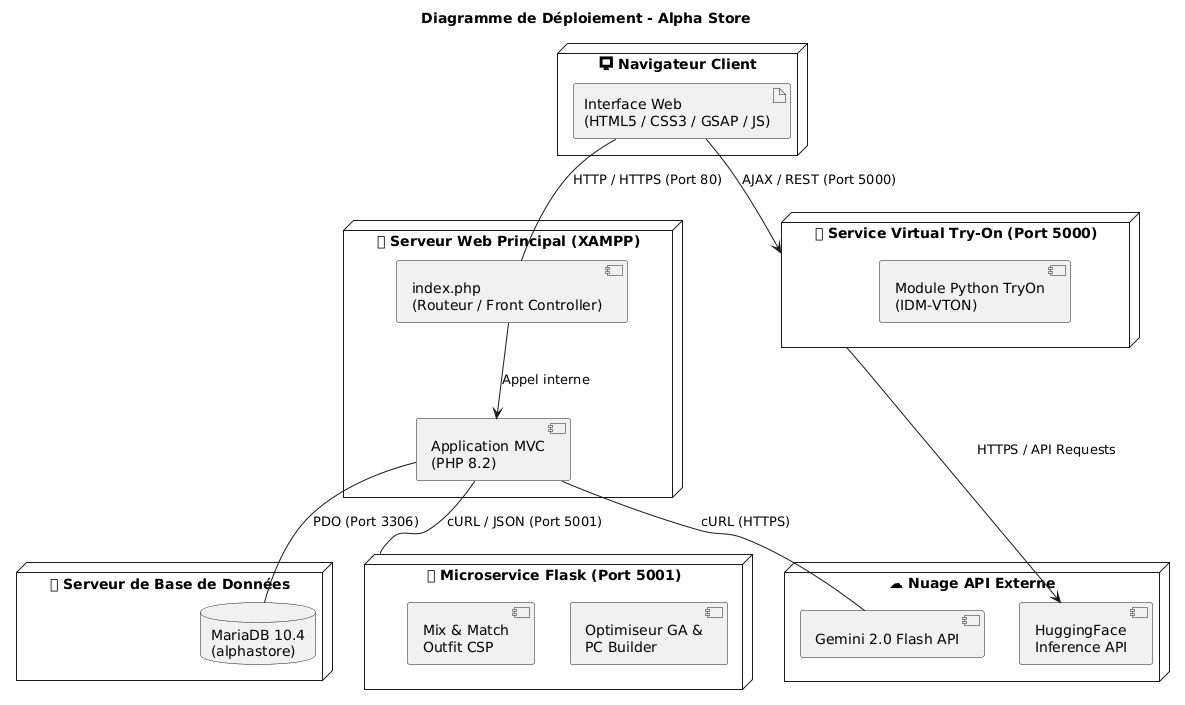
\includegraphics[width=0.85\textwidth]{chapitre3/figuresChap3/deployment diagram.png}
    \caption{Diagramme de déploiement d'Alpha Store}
    \label{fig:deployment}
\end{figure}

\subsection{Diagramme de classes}

Le diagramme de classes montre les principales entités du système et leurs relations, telles que Utilisateur, Produit, Commande, Panier, Favoris et IA.

\begin{figure}[H]
    \centering
    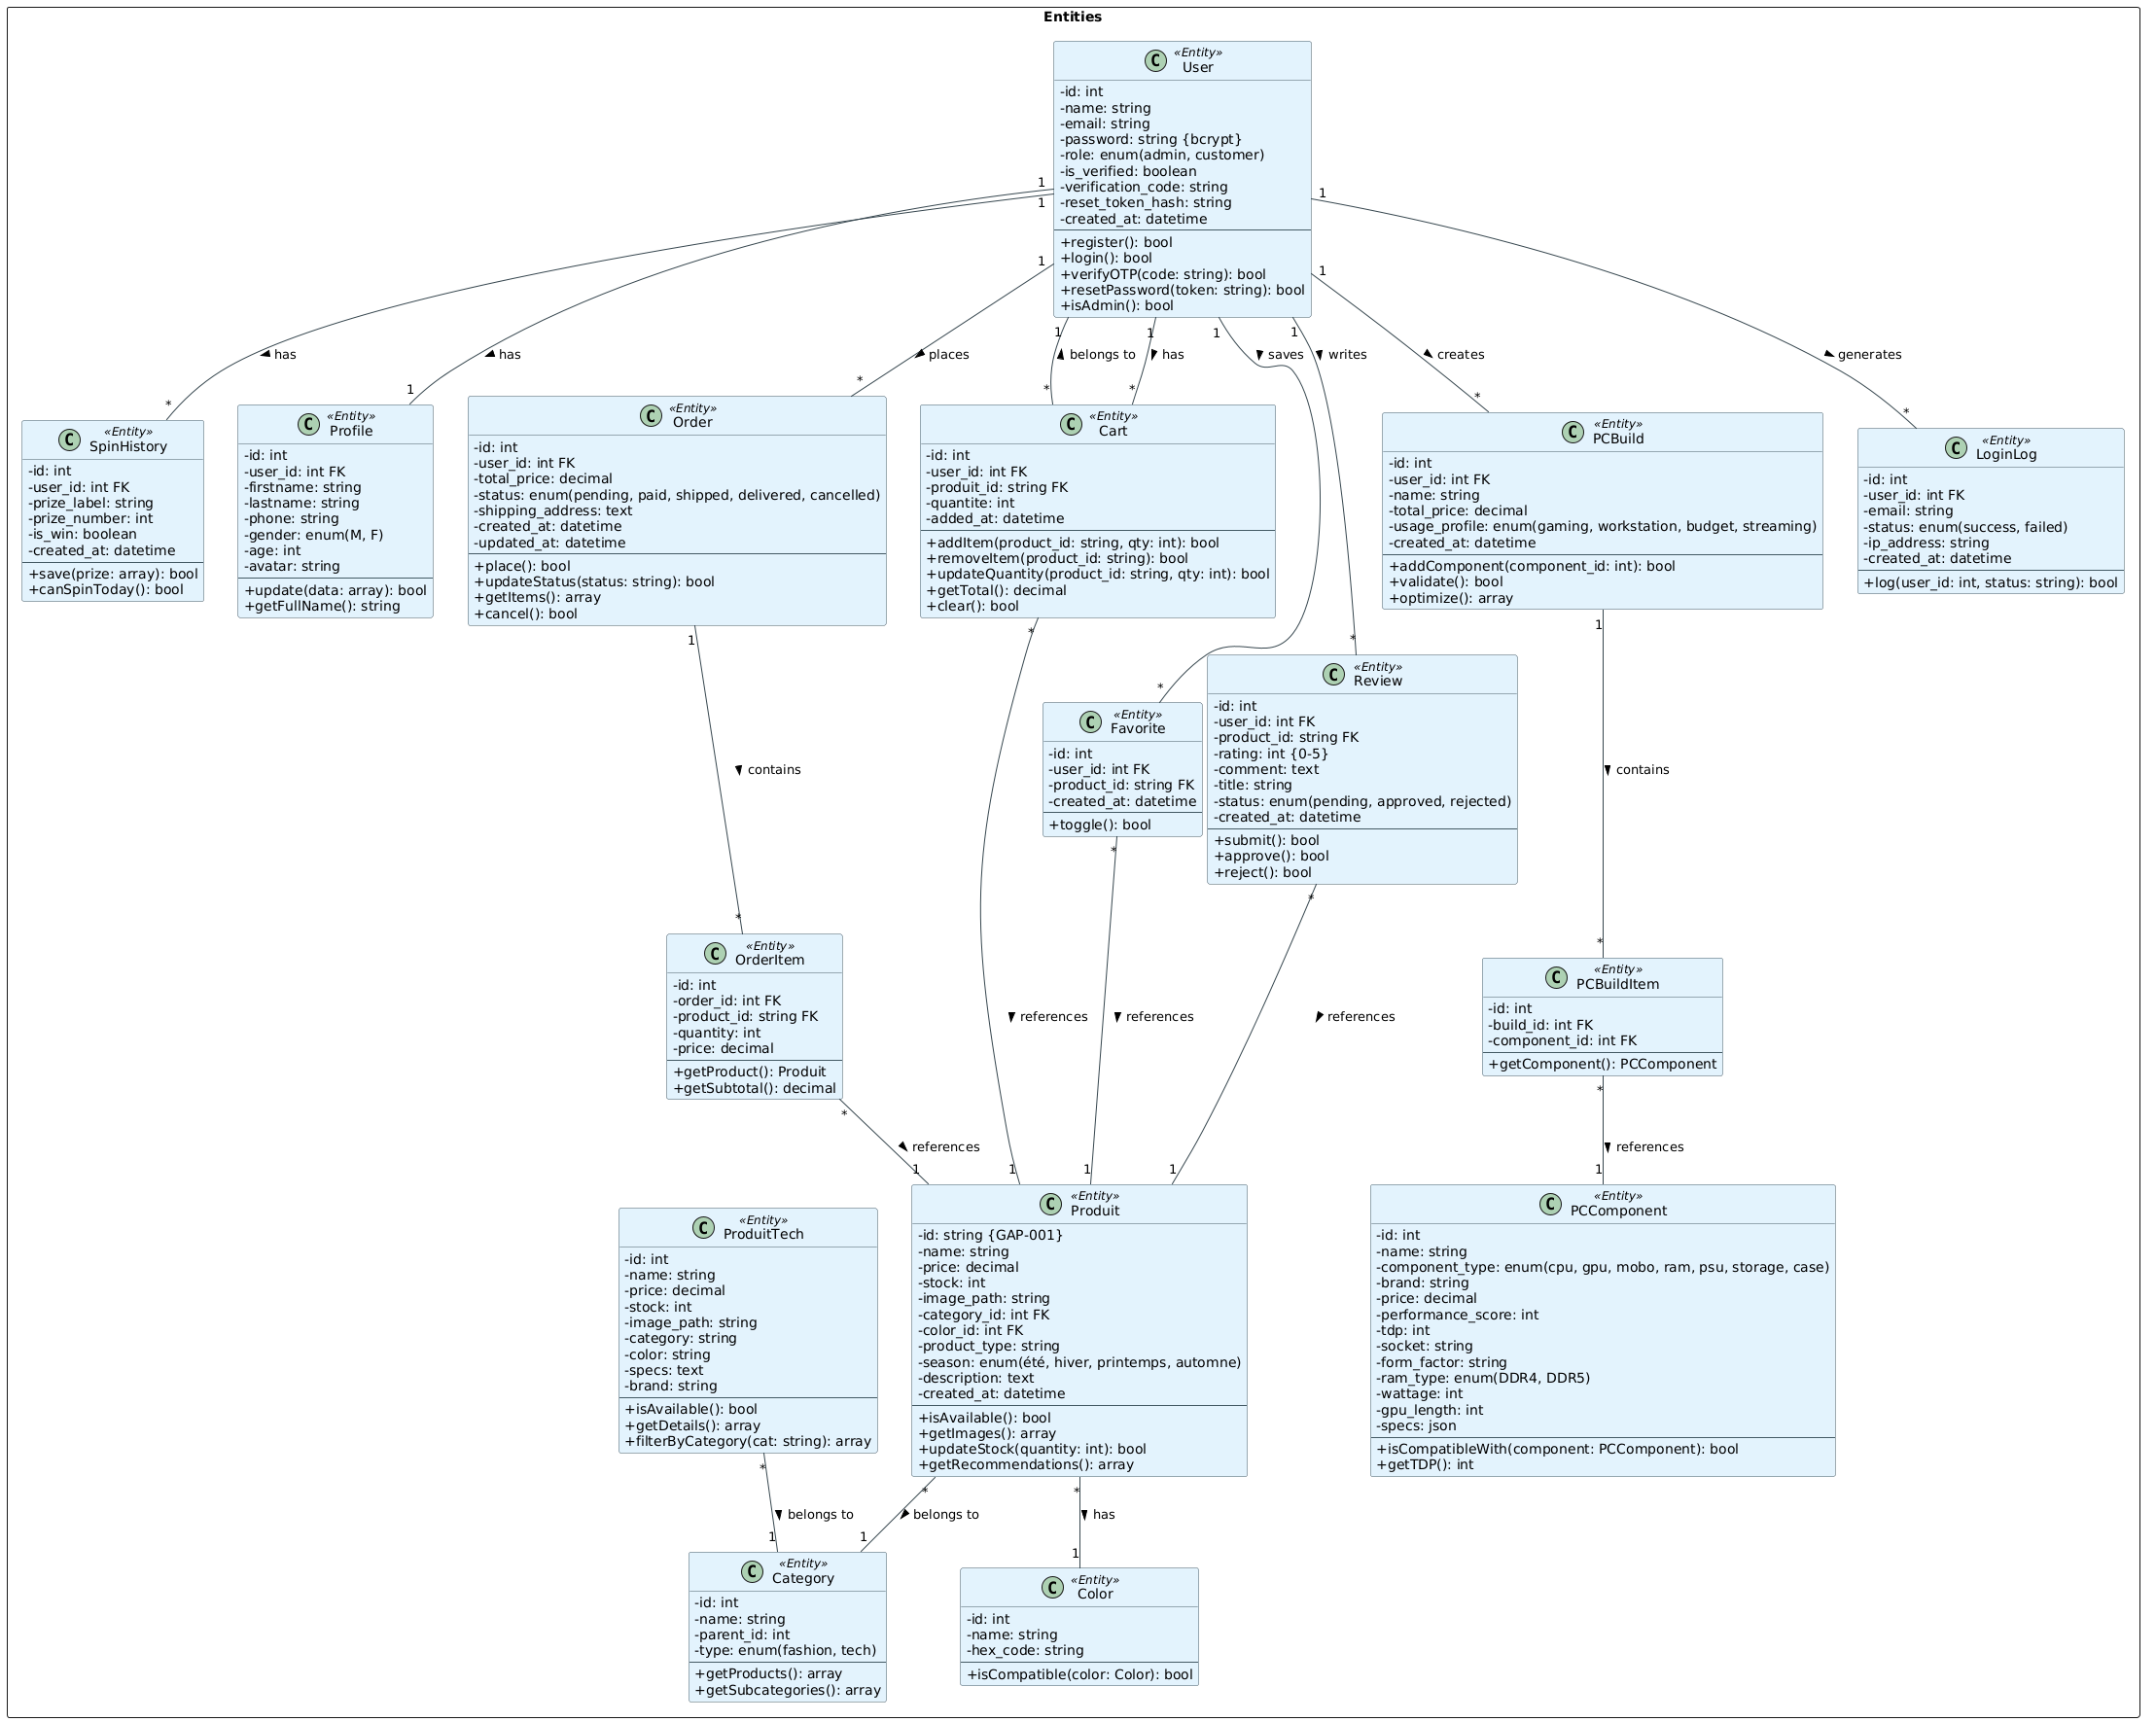
\includegraphics[width=0.95\textwidth]{chapitre3/figuresChap3/diagramme de classe partie 1.png}
    \caption{Diagramme de classes global d'Alpha Store}
    \label{fig:class_diagram}
\end{figure}
\begin{figure}[H]
    \centering
    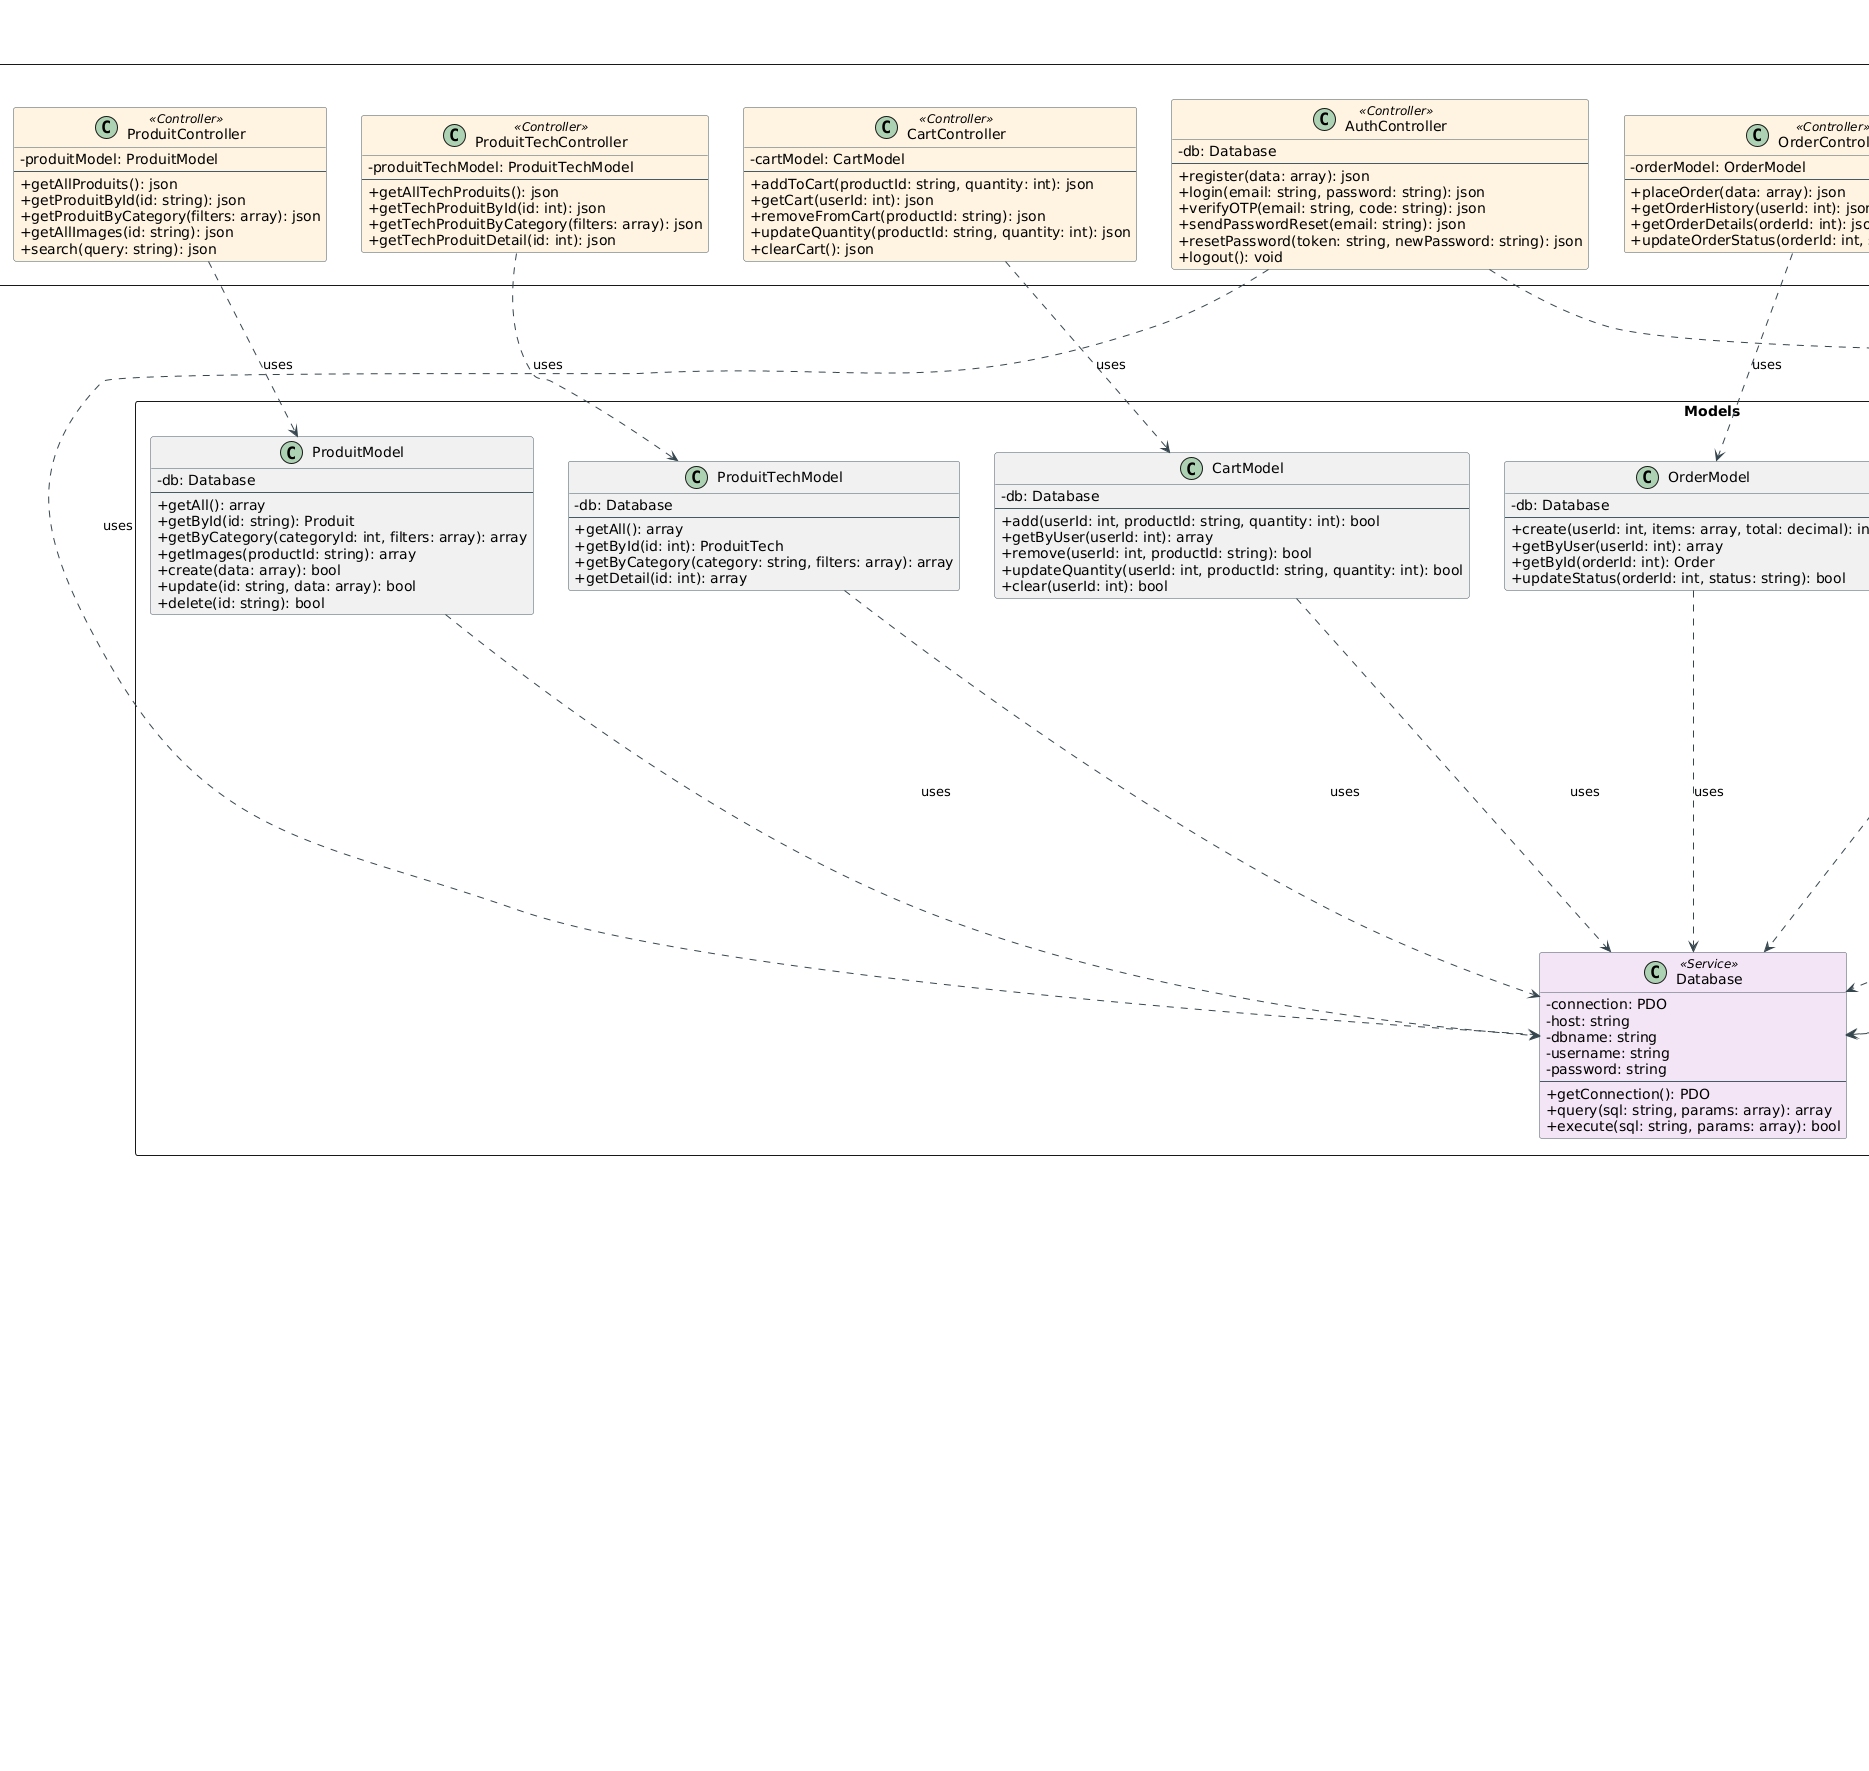
\includegraphics[width=0.95\textwidth]{chapitre3/figuresChap3/digramme de classe partie 2 (modele,controller).png}
    \caption{Diagramme de classes pour modele et connroller}
    \label{fig:class_diagram}
\end{figure}
\section{Conception : vue dynamique}

La vue dynamique illustre le comportement du système à travers des scénarios d'utilisation importants, en mettant l'accent sur les échanges entre objets et services.

\subsection{Diagrammes de séquence}

Pour chaque fonctionnalité étudiée, nous présentons un diagramme de séquence système (niveau macro) et un diagramme de séquence détaillé (niveau micro).

\subsubsection{Diagramme de séquence << Passer une commande >>}

\begin{itemize}[label=$\bullet$]
    \item \textbf{Diagramme système}
    \begin{figure}[H]
        \centering
        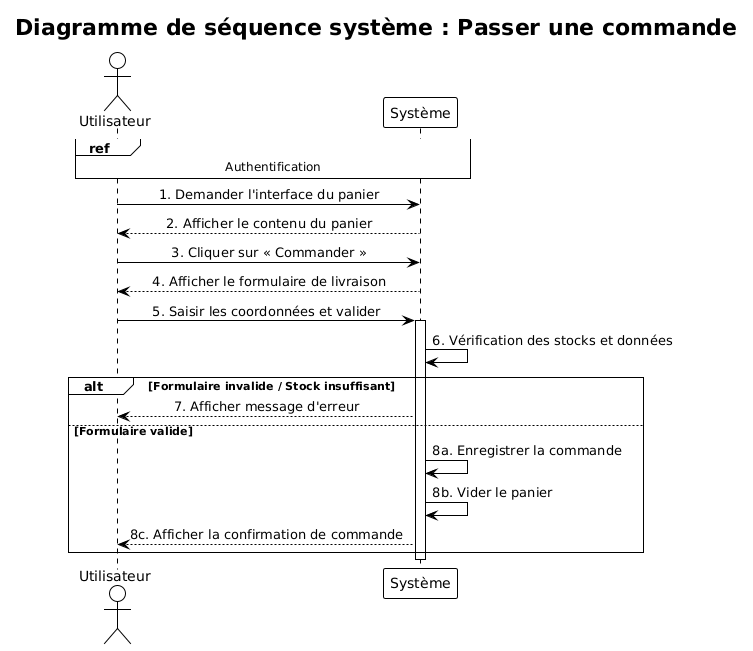
\includegraphics[width=0.75\textwidth]{chapitre3/figuresChap3/Passer une commande.png}
        \caption{Diagramme système : Passer une commande}
        \label{fig:cmd_sys}
    \end{figure}

    \item \textbf{Diagramme détaillé}
    \begin{figure}[H]
        \centering
        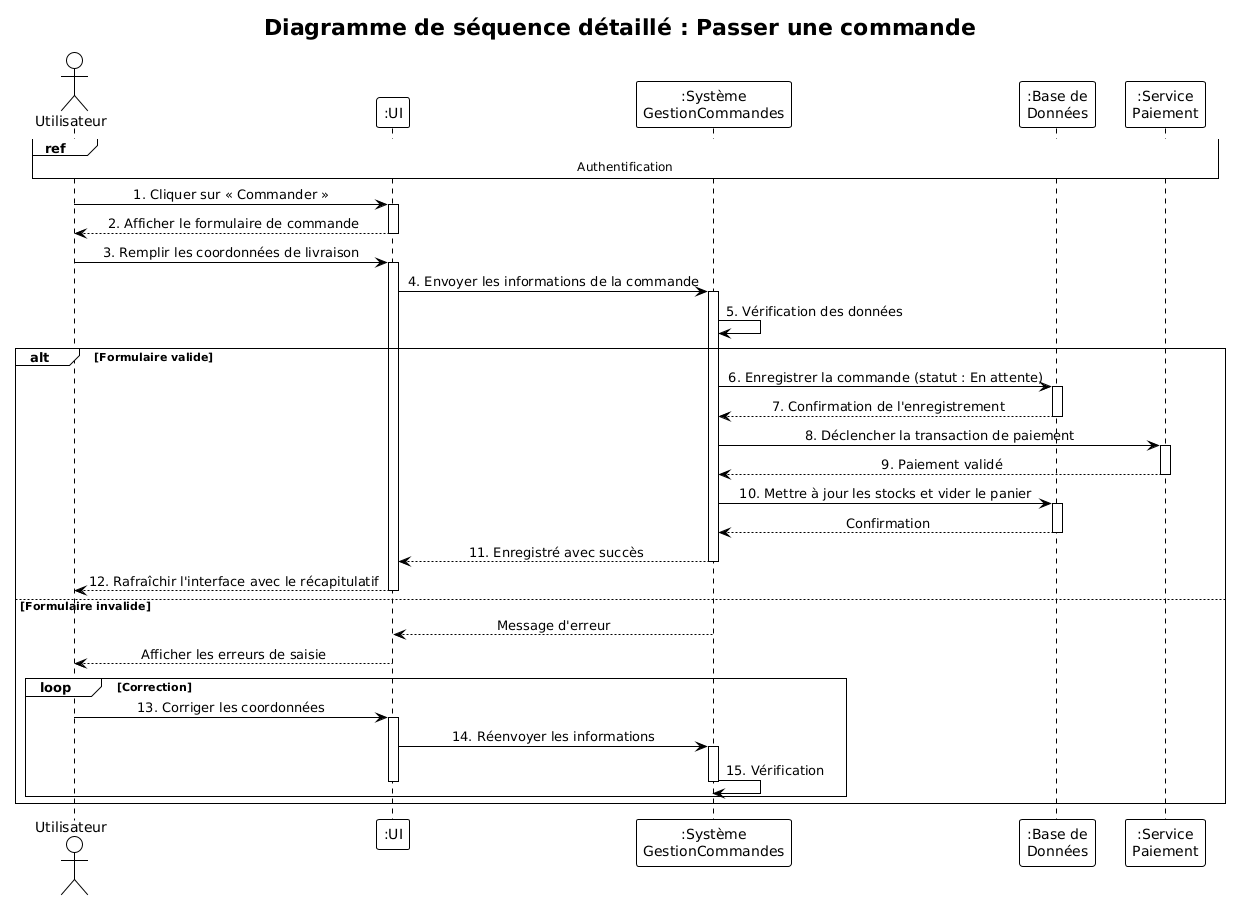
\includegraphics[width=0.75\textwidth]{chapitre3/figuresChap3/Passer une commande1.png}
        \caption{Diagramme détaillé : Passer une commande}
        \label{fig:cmd_detail}
    \end{figure}
\end{itemize}

La figure \ref{fig:cmd_sys} (diagramme système) présente le flux global : le client valide son panier via l'interface, le front-end transmet la commande au `OrderController` qui orchestre la création de la commande, invoque le service de paiement externe et met à jour la base de données. La figure \ref{fig:cmd_detail} (diagramme détaillé) précise les échanges entre `Cart`, `Order`, `InventoryService`, `PaymentService`, `Database` et `Mailer` : vérification de stock, création d'un enregistrement `Order`, réservation du stock, traitement du paiement et notification par e-mail.

\subsubsection{Diagramme de séquence << Essayage virtuel >>}

\begin{itemize}[label=$\bullet$]
    \item \textbf{Diagramme système}
    \begin{figure}[H]
        \centering
        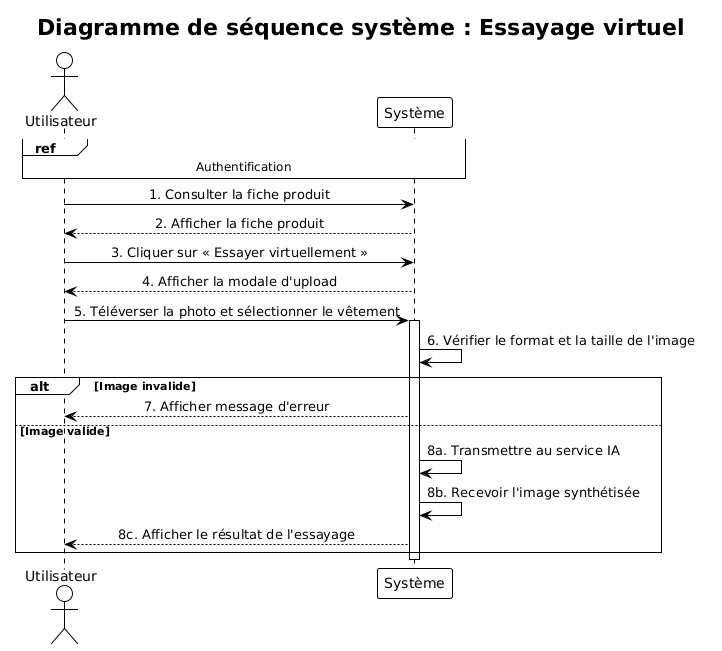
\includegraphics[width=0.75\textwidth]{chapitre3/figuresChap3/Essayage virtuel.png}
        \caption{Diagramme système : Essayage virtuel}
        \label{fig:tryon_sys}
    \end{figure}

    \item \textbf{Diagramme détaillé}
    \begin{figure}[H]
        \centering
        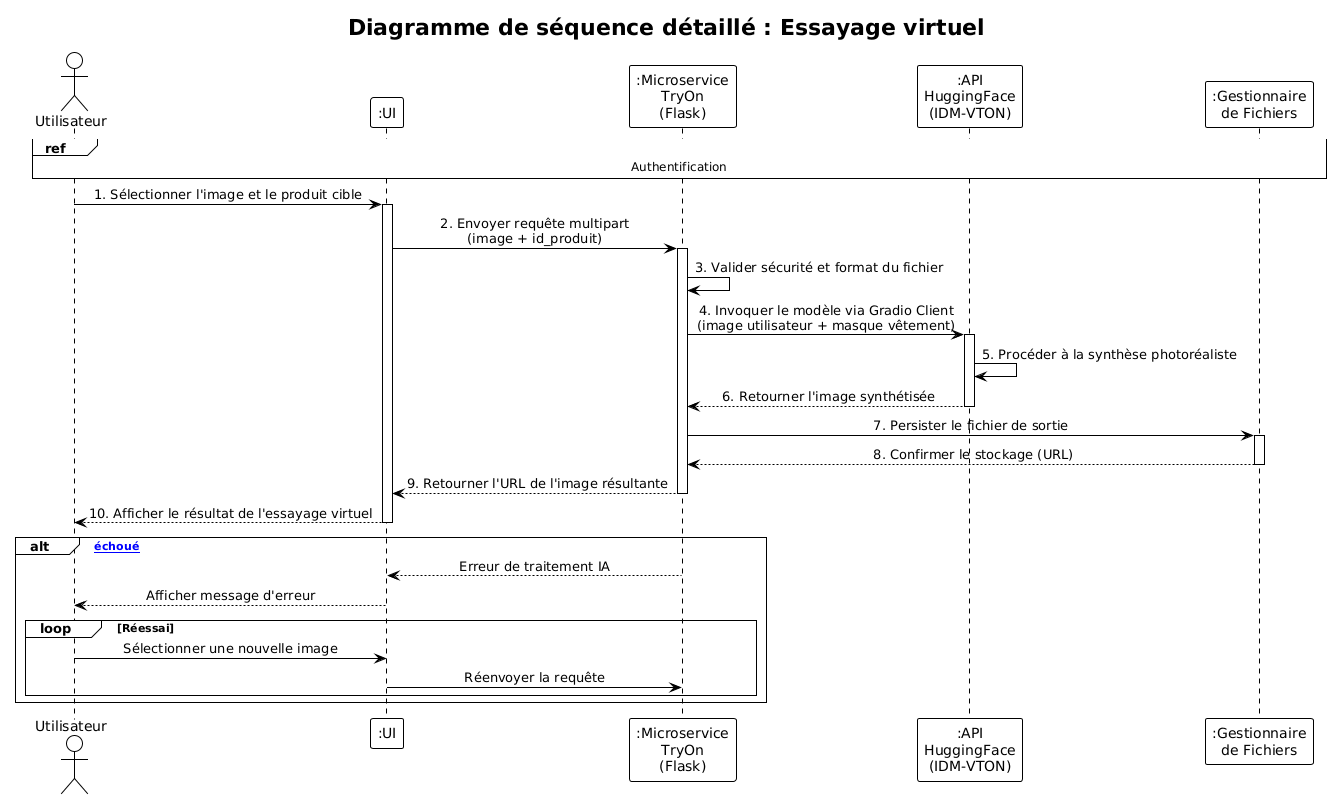
\includegraphics[width=0.75\textwidth]{chapitre3/figuresChap3/Essayage virtuel1.png}
        \caption{Diagramme détaillé : Essayage virtuel}
        \label{fig:tryon_detail}
    \end{figure}
\end{itemize}

La figure \ref{fig:tryon_sys} décrit le flux macro : l'utilisateur télécharge une photo et sélectionne un vêtement, l'interface envoie la requête au `TryOnController` qui appelle le microservice Try-On (Flask) et, si besoin, l'API d'inférence externe (HuggingFace IDM-VTON). La figure \ref{fig:tryon_detail} explicite les étapes techniques : pré-traitement de l'image, appel à l'API d'inférence, post-traitement (masques, ajustements), stockage temporaire et retour de l'image composite à l'interface.

\subsubsection{Diagramme de séquence << build pc >>}

\begin{itemize}[label=$\bullet$]
    \item \textbf{Diagramme système}
    \begin{figure}[H]
        \centering
        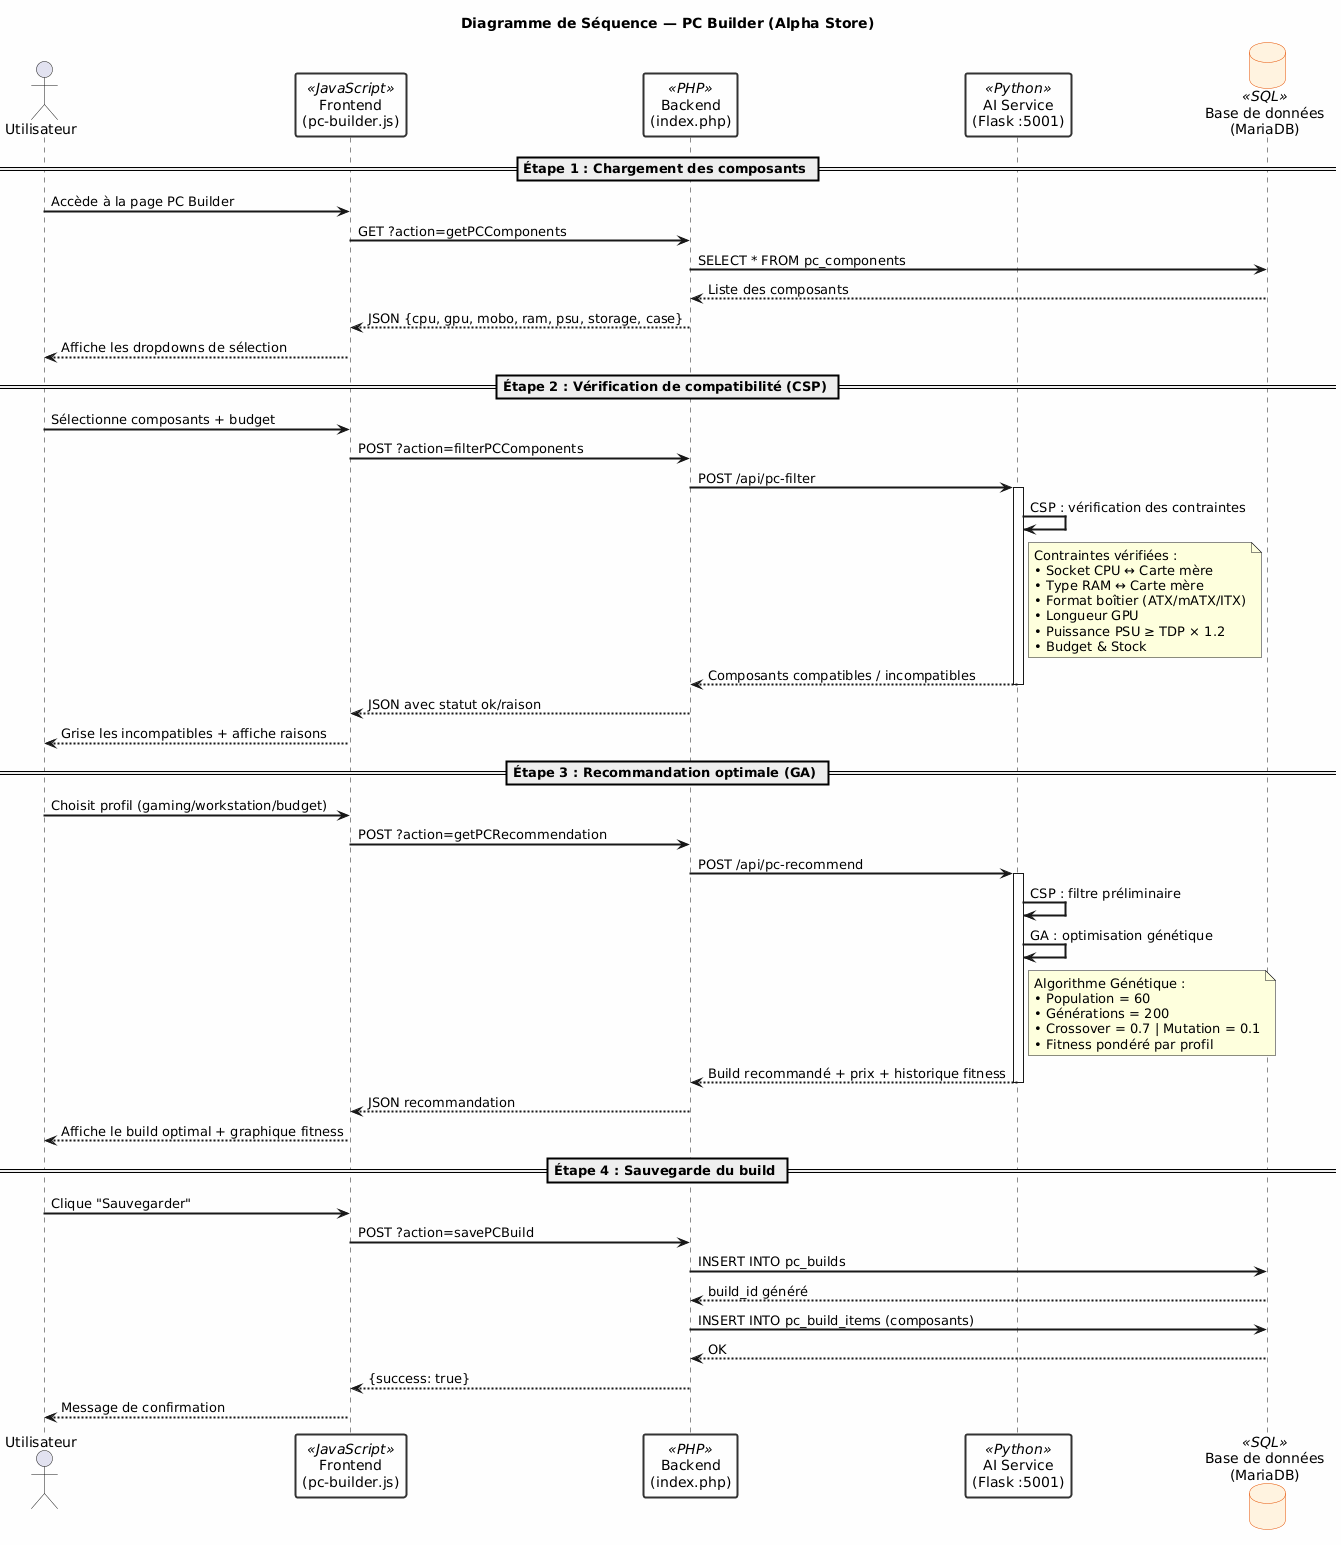
\includegraphics[width=0.75\textwidth]{chapitre3/figuresChap3/PCBuilder.png}
        \caption{Diagramme système : build pc}
        \label{fig:pc_sys}
    \end{figure}

    \item \textbf{Diagramme détaillé}
    \begin{figure}[H]
        \centering
        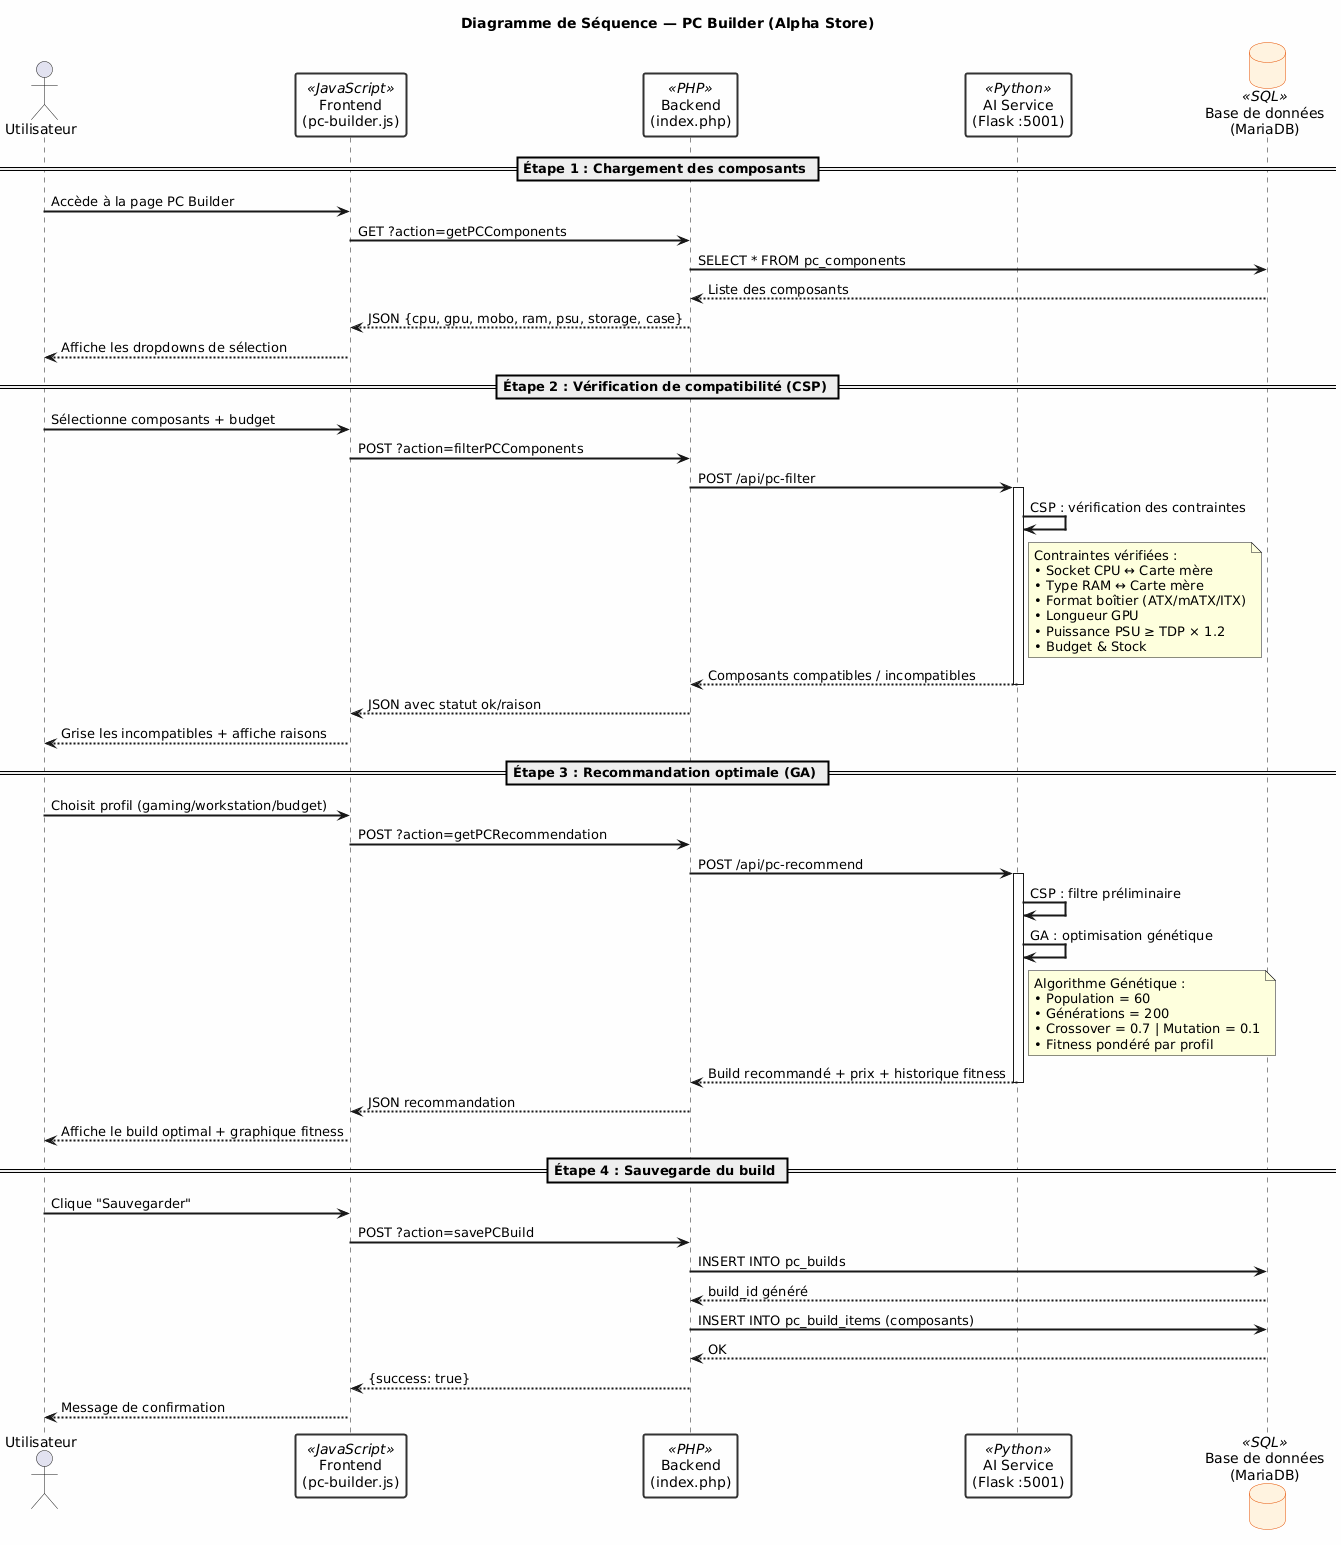
\includegraphics[width=0.75\textwidth]{chapitre3/figuresChap3/PCBuilder.png}
        \caption{Diagramme détaillé : build pc}
        \label{fig:pc_detail}
    \end{figure}
\end{itemize}

\subsection{Diagramme d'activité : Algorithme Génétique (PC Builder / Smart Budget)}

Pour garantir une optimisation robuste sous contraintes multiples (respect strict du budget de l'utilisateur et compatibilité matérielle absolue telle que le socket du processeur vs la carte mère), le comportement interne de notre composant d'intelligence artificielle est modélisé par un diagramme d'activité UML.

Le flux suit les étapes clés du cycle évolutionnaire :

\begin{itemize}[label=$\bullet$]
    \item \textbf{Initialisation :} Lecture du budget maximum fixé par l'utilisateur et génération d'une population initiale de configurations (chromosomes) aléatoires, mais respectant le filtrage préliminaire de compatibilité (CSP).
    \item \textbf{Évaluation (Calcul de la Fitness) :} Chaque configuration se voit attribuer un score de performance globale. Si la configuration dépasse le budget ou présente une anomalie, elle reçoit une pénalité éliminatoire.
    \item \textbf{Sélection \& Croisement :} Les meilleures configurations (les plus adaptées au budget et performantes) sont sélectionnées pour former un bassin de reproduction. Elles s'échangent des gènes (composants) pour créer des descendants potentiellement meilleurs.
    \item \textbf{Mutation :} Une altération aléatoire faible est introduite (changement d'une barrette mémoire ou d'un stockage) pour explorer de nouvelles solutions et éviter la convergence prématurée.
    \item \textbf{Critère d'arrêt :} Le cycle se répète jusqu'à ce que la solution optimale stagne sur un nombre défini de générations ou que le nombre maximal d'itérations soit atteint. La meilleure configuration finale est alors renvoyée à l'interface utilisateur.
\end{itemize}

\begin{figure}[H]
    \centering
    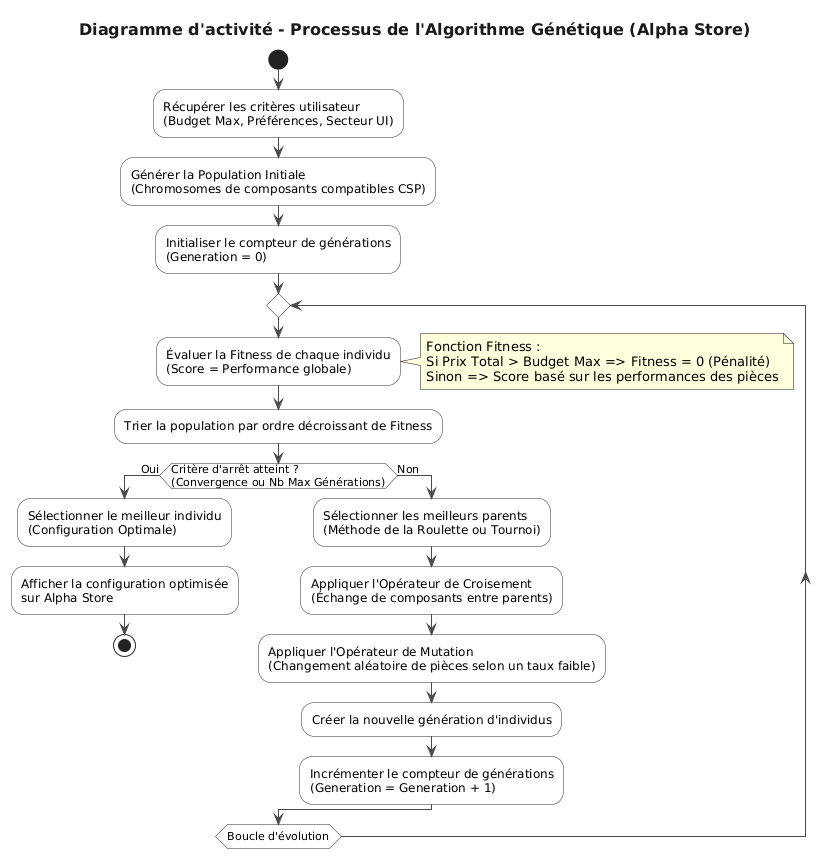
\includegraphics[width=0.8\textwidth]{chapitre3/figuresChap3/AlgorithmeGénétique.png}
    \caption{Diagramme d'activité de l'Algorithme Génétique}
    \label{fig:ga_activity}
\end{figure}


La figure \ref{fig:pc_sys} donne une vue d'ensemble : l'utilisateur choisit ou renseigne des contraintes (budget, usage), le `PCBuildController` consulte le service CSP pour filtrer la compatibilité et le service GA pour proposer une configuration optimisée, puis renvoie la configuration au client. La figure \ref{fig:pc_detail} précise les échanges entre `PCBuilderUI`, `PCBuildController`, `PC_CSP_Service`, `PC_GA_Service`, `PCComponentsRepository` et `Session` : validation des compatibilités (socket, RAM, format), optimisation, génération de l'objet `PCBuild` et enregistrement de la proposition.

\section{Diagramme d'état/transition}

La modélisation par diagramme d'état/transition décrit les différents états d'un objet et les transitions qui les relient. Cela permet de clarifier le comportement interne et les flux possibles.

\subsection{Diagramme d'état/transition : objet commande}

Le diagramme d'état/transition de l'objet commande illustre le cycle de vie complet d'une commande au sein de la plateforme Alpha Store. Il retrace l'évolution de l'état de la commande depuis sa création initiale dans le panier du client jusqu'à sa livraison finale ou son éventuelle annulation. Les différentes transitions sont déclenchées par les actions du client (validation, paiement) ou par les mises à jour effectuées par l'administrateur (expédition, livraison). Ce formalisme permet de s'assurer que chaque étape du processus e-commerce est correctement gérée et suivie.

\begin{figure}[H]
    \centering
    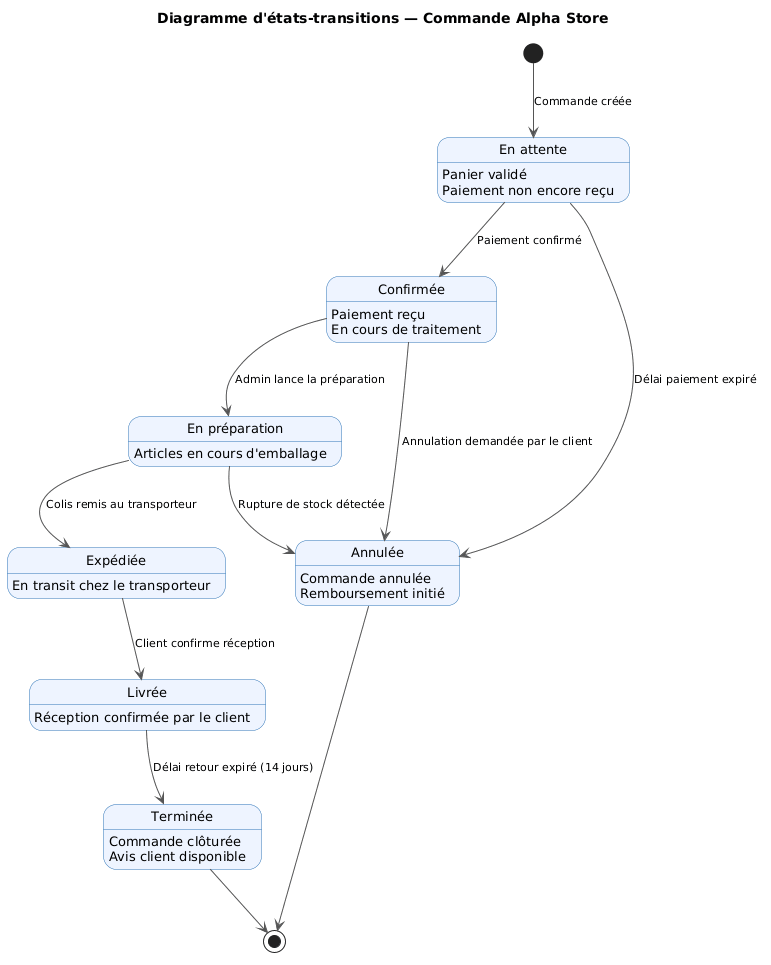
\includegraphics[width=0.85\textwidth]{chapitre3/figuresChap3/etat_commande.png}
    \caption{Diagramme d'état/transition de l'objet commande}
    \label{fig:etat_commande}
\end{figure}

\section{Conclusion}

Ce chapitre a présenté l'étude conceptuelle d'Alpha Store en combinant une vue statique et une vue dynamique. La structure logicielle et l'architecture physique ont été décrites, tandis que les scénarios de séquence ont permis de valider les principaux comportements attendus. Ces éléments serviront de référence pour la phase de réalisation.
